% Number 150
% CVPMG Units
% Problem-solving, Creed and Kevin on bikes
% JG

% Watermark
\AddToShipoutPicture*{\BackgroundPic}

\addtocounter {ProbNum} {1}

%\begin{floatingfigure}[r]{.3\textwidth}
%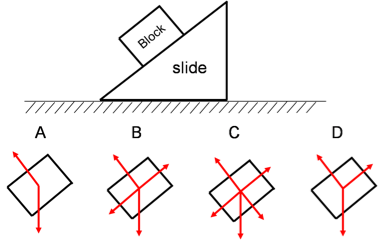
\includegraphics[scale=.4]{/Users/jgates/desktop/latex/pics/incline3.png}
%\end{floatingfigure}
 
{\bf \Large{\arabic{ProbNum}}} Creed and Kevin find some bikes by the loading dock, and devise a competition: they use an 8 meter long rope to tie their bikes together and set up next to each other, facing opposite directions.  They begin next to each other, start their pedaling at the same time and ride in opposite directions, trying to see who can ride the furthest before the rope snaps tight. If Creed can pedal his bike at 4 meters per second, and he ends up 5.1 meters away from the starting point, how fast did Kevin pedal?  Solve it graphically!  Assume that they can get up to speed instantly.

%\bigskip

%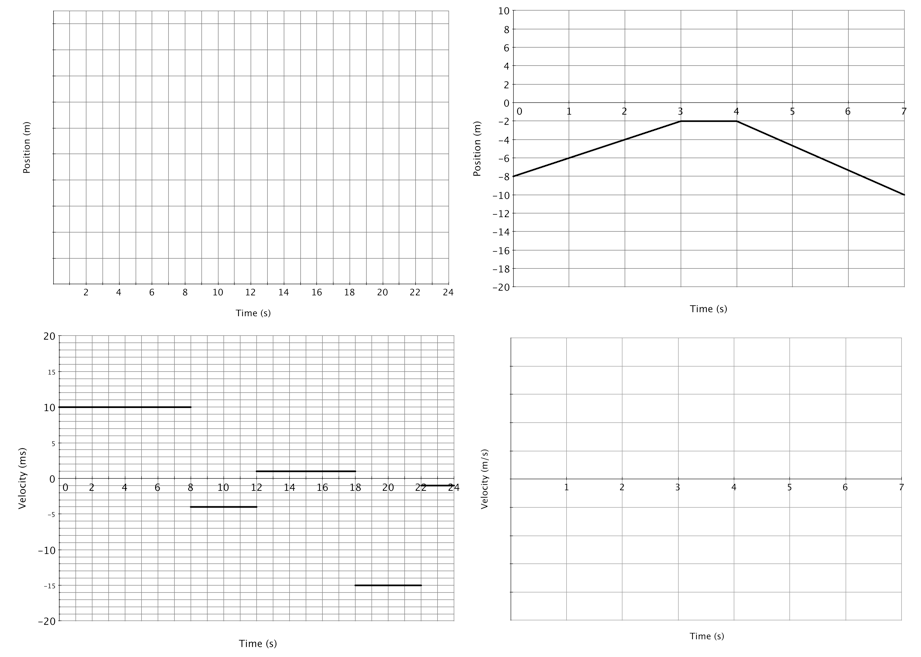
\includegraphics[scale=.57]{/Users/jgates/desktop/latex/pics/cvpmgraphs1.png}

\vfill

\newpage
